\chapter{Конструкторская часть}

\section{Функции принадлежности}

Для введения нечёткости предлагается рассматривать нечёткие переменные <<скорость>> (автопилота) и <<расстояние>> (до лидера) и задавать их с помощью функций принадлежности термам <<очень низкая(ое)>>, <<низкая(ое)>>, <<средняя(ее)>>, <<высокая(ое)>> и <<очень высокая(ое)>>. Графики предлагаемых функций принадлежности представлены на рисунках \ref{img:v} и \ref{img:s}.

\begin{figure}[h!]
	\begin{center}
		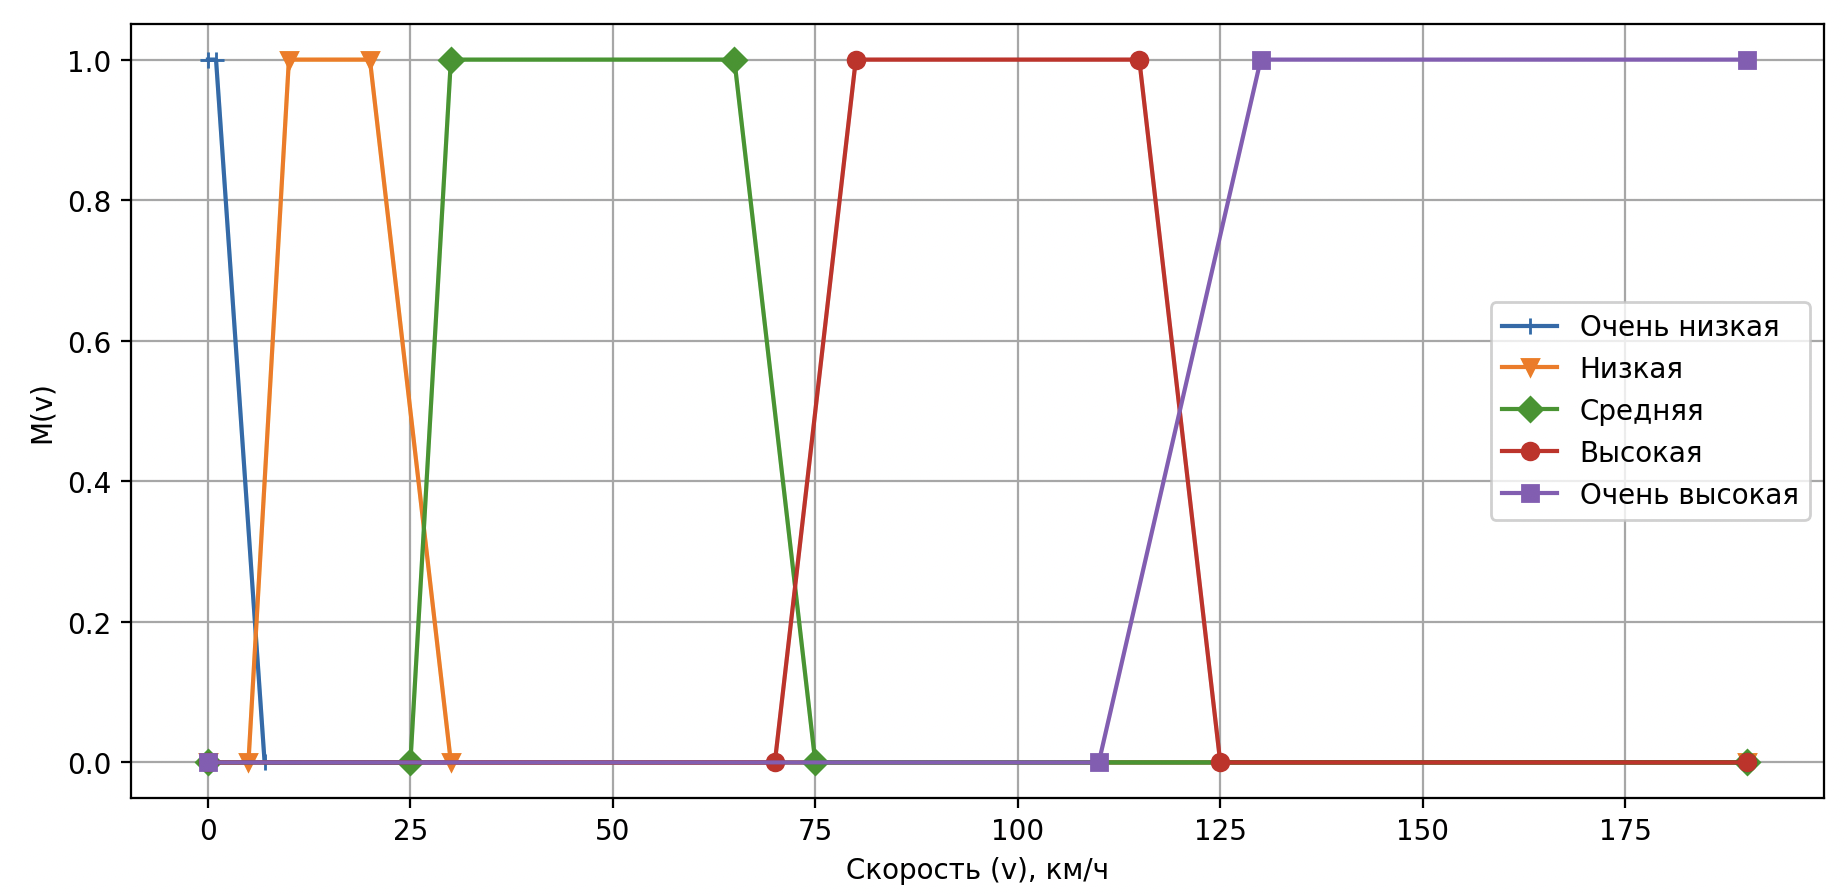
\includegraphics[width=\textwidth]{images/v.png}
	\end{center}
	\caption{Графики функций принадлежности термам значений скорости}
	\label{img:v}
\end{figure}

\begin{figure}[h!]
	\begin{center}
		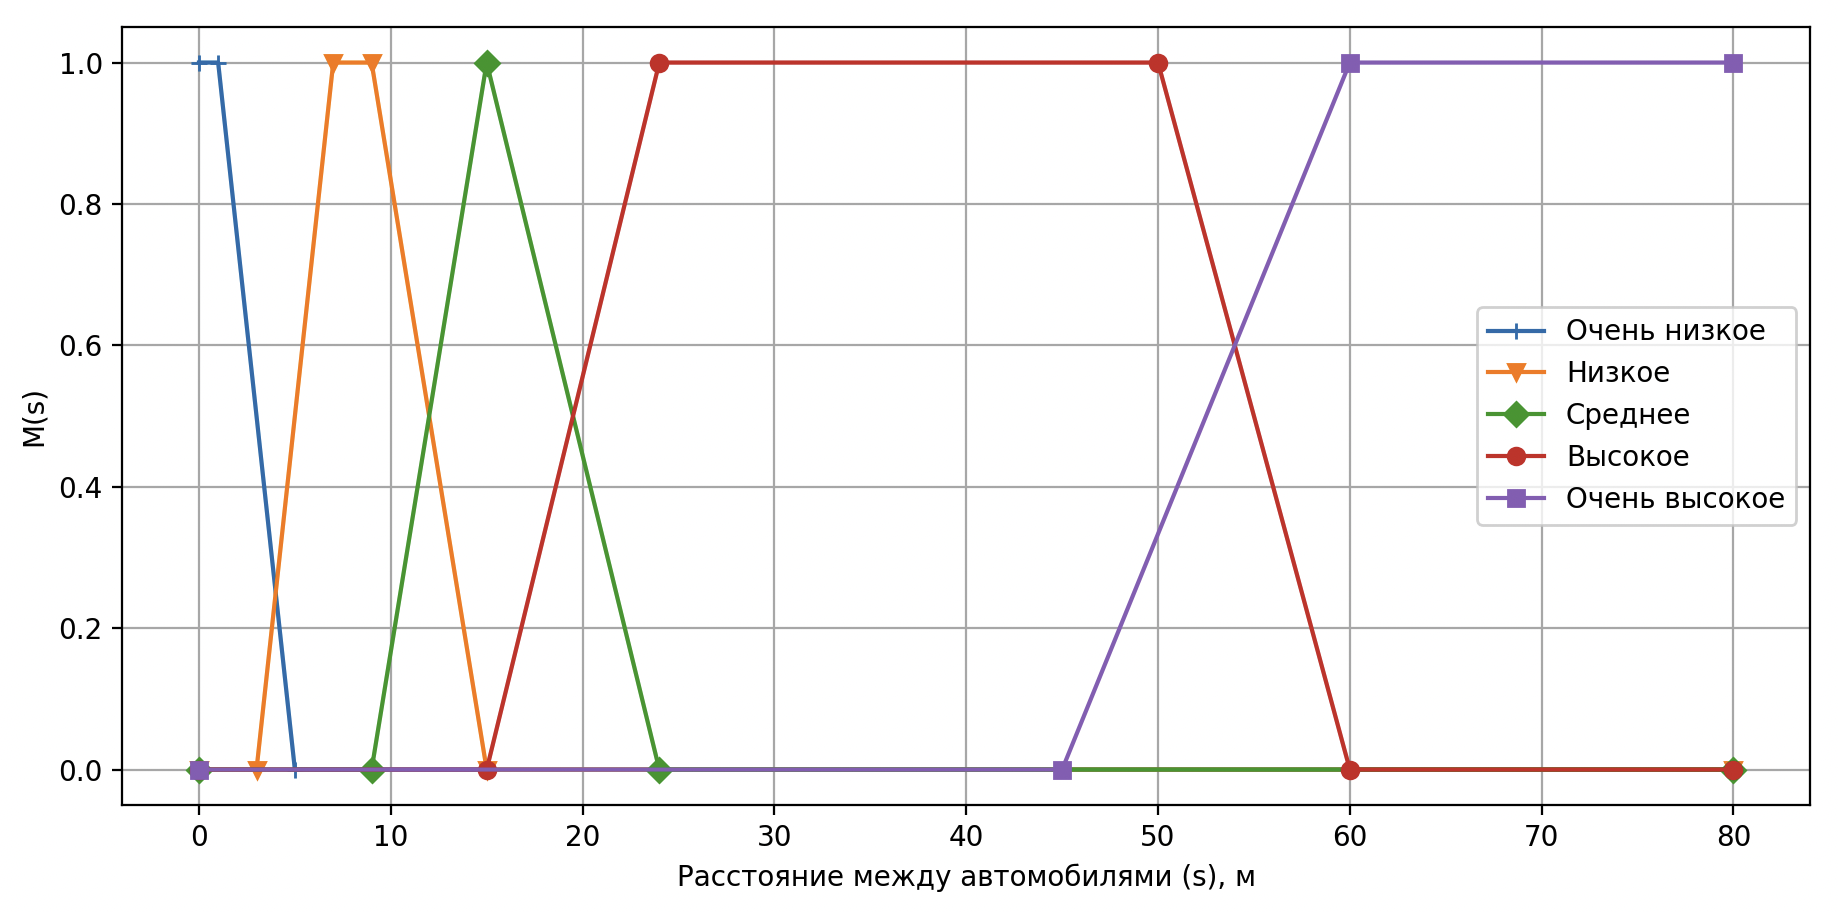
\includegraphics[width=\textwidth]{images/s.png}
	\end{center}
	\caption{Графики функций принадлежности термам значений расстояния между лидером и автопилотом}
	\label{img:s}
\end{figure}

Функция принадлежности расстояния терму <<среднее>> имеет единственный максимум, достигаемый при расстоянии равным 15 метров. Таким образом задаётся фиксированное расстояние до лидера, которого должен строго придерживаться автопилот.

\section{База правил}

Для определения рекомендуемой скорости автопилота была разработана база правил вида \ref{rule}. Предлагаемые правила представлены в таблице \ref{tab:labels}

\begin{table}[H]
	\centering
	\caption{Зависимость рекомендуемой скорости автопилота от его текущей скорости и его расстояния до лидера}
	\label{tab:labels}
	\renewcommand{\arraystretch}{1.7}
	\begin{tabular}{cc|c|c|c|c|c|}
		\cline{3-7}
		& & \multicolumn{5}{ c| }{Текущая скорость автопилота} \\ \cline{3-7}
		& & \parbox{1.3cm}{\linespread{0.8}\selectfont Очень\\низкая} & Низкая & Средняя & Высокая & \parbox{1.5cm}{\linespread{0.8}\selectfont Очень\\высокая} \\ \cline{1-7}
		\multicolumn{1}{ |c  }{\multirow{5}{*}{\rotatebox[origin=c]{90}{\parbox{2cm}{\linespread{0.8}\selectfont Расстояние\\до лидера}} } } &
		\multicolumn{1}{ |c| }{\parbox{1.3cm}{\linespread{0.8}\selectfont Очень\\низкое}} & \parbox{1.3cm}{\linespread{0.8}\selectfont Очень\\низкая} & \parbox{1.3cm}{\linespread{0.8}\selectfont Очень\\низкая} & \parbox{1.3cm}{\linespread{0.8}\selectfont Очень\\низкая} & \parbox{1.3cm}{\linespread{0.8}\selectfont Очень\\низкая} & \parbox{1.3cm}{\linespread{0.8}\selectfont Очень\\низкая}  \\ \cline{2-7}
		\multicolumn{1}{ |c  }{}                        &
		\multicolumn{1}{ |c| }{Низкое} & \parbox{1.3cm}{\linespread{0.8}\selectfont Очень\\низкая} & \parbox{1.3cm}{\linespread{0.8}\selectfont Очень\\низкая} & Низкая & Низкая & Низкая  \\ \cline{2-7}
		\multicolumn{1}{ |c  }{} &
		\multicolumn{1}{ |c| }{Среднее} & \parbox{1.3cm}{\linespread{0.8}\selectfont Очень\\низкая} & Низкая & Средняя & Средняя & Высокая \\ \cline{2-7}
		\multicolumn{1}{ |c  }{}                        &
		\multicolumn{1}{ |c| }{Высокое} & Низкая & Средняя & Высокая & Высокая & \parbox{1.5cm}{\linespread{0.8}\selectfont Очень\\высокая} \\ \cline{2-7}
		\multicolumn{1}{ |c  }{}                        &
		\multicolumn{1}{ |c| }{\parbox{1.5cm}{\linespread{0.8}\selectfont Очень\\высокое}} & Средняя & Средняя & Высокая & \parbox{1.5cm}{\linespread{0.8}\selectfont Очень\\высокая} & \parbox{1.5cm}{\linespread{0.8}\selectfont Очень\\высокая} \\ \cline{1-7}
	\end{tabular}
\end{table}

\section*{Вывод}

В данном разделе были предложены функции принадлежности термам числовых значений скорости автопилота и его расстояния до лидера, а также правила для нечёткого логического вывода.

\clearpage
